\section{VALIDACIÓN DE LA SOLUCIÓN}

El presente capítulo tiene como objetivo fundamental comprobar la eficacia de la solución metodológica y tecnológica propuesta. Para someter el sistema a una prueba rigurosa, se estableció un marco experimental basado en el procesamiento de adquisiciones controladas de resonancia magnética. 

La demostración empírica de la propuesta se divide en dos ejes principales de evaluación:

\begin{itemize}
    \item \textbf{Verificación del procesamiento espacial y acústico (Etapas \ref{item:etapa1} y \ref{item:etapa2}):} Consiste en verificar el correcto desempeño operativo de los módulos de \textit{software}. Se analizan los resultados de la adaptación espacial y de la síntesis de audio, corroborando que el sistema logra aislar la anatomía del fantoma y transformar exitosamente su cinemática en señales sonoras y espectrogramas representativos.

    
    \item \textbf{Validación estadística y perceptiva (Etapa 3):} Se centra en la comparación y capacidad discriminatoria del modelo sobre los datos generados. Inicia con un análisis cuantitativo apoyado en técnicas de aprendizaje no supervisado para medir la separación estadística de las métricas. Culmina con una validación cualitativa en el entorno interactivo, demostrando que el contraste de estas sonificaciones permite identificar firmas acústicas distinguibles frente a variaciones del flujo.
\end{itemize}


\subsection{Caracterización de los datos experimentales}

Previa a la exposición de los resultados, es necesario detallar las características del conjunto de datos de prueba utilizado. El marco experimental está compuesto por adquisiciones de \textit{4D Flow MRI} correspondientes a fantomas cardiovasculares. En el ámbito de la hemodinámica, un fantoma es un modelo físico calibrado diseñado específicamente para emular la geometría del sistema cardiovascular.

Para evaluar la capacidad de respuesta del sistema ante alteraciones complejas, el conjunto de pruebas contempló modelos con distintos grados de coartación, un estrechamiento anatómico del vaso que obliga al fluido a acelerarse abruptamente y generar turbulencia. Al procesar diferentes diámetros para esta lesión, se busca verificar si el algoritmo logra capturar y parametrizar acústicamente los diferentes escenarios.

Para comprobar que el modelo acústico es capaz de distinguir diferentes niveles de intensidad hemodinámica, las geometrías fueron sometidas a dos condiciones de flujo contrastantes:

\begin{itemize}
    \item \textbf{Condición de reposo (\textit{rest}):} Emula el comportamiento fisiológico basal, definiendo un patrón de velocidades no alterado por factores externos.
    
    \item \textbf{Condición de estrés (\textit{stress}):} Representa un estado de alta demanda cardiovascular, el cual fuerza un aumento drástico en las velocidades en el flujo.
\end{itemize}

Las configuraciones que definen los escenarios de estudio evaluados se resumen en la Tabla \ref{table:casos_estudio}.

\begin{table}[h]
    \centering
    \caption{\label{table:casos_estudio} Conjunto de datos evaluados en la experimentación.}
    \begin{tabular}{|l|l|}
        \hline
        \textbf{Geometría del Fantoma} & \textbf{Condiciones Evaluadas} \\
        \hline
        Normal & Reposo (\textit{rest}), Estrés (\textit{stress}) \\
        \hline
        13 mm & Reposo (\textit{rest}), Estrés (\textit{stress}) \\
        \hline
        11 mm & Reposo (\textit{rest}), Estrés (\textit{stress}) \\
        \hline
        9 mm & Reposo (\textit{rest}), Estrés (\textit{stress}) \\
        \hline
    \end{tabular}
\end{table}


Definidos los ocho escenarios de estudio, la primera fase de validación aborda el desempeño de los módulos de procesamiento espacial y acústico. Considerando que los volúmenes hemodinámicos, las segmentaciones y los \textit{centerlines} se proporcionan como datos de entrada, el objetivo de esta etapa es demostrar la correcta integración y transformación de estos elementos. A continuación, se verifica la capacidad del algoritmo para iterar sobre la trayectoria anatómica y extraer los perfiles de velocidad locales, para finalmente exhibir cómo esta cinemática se convierte exitosamente en las señales sonoras y espectrogramas representativos del fantoma.


\subsection{Verificación del procesamiento espacial y acústico}

La verificación de este flujo de trabajo se expone en dos partes. Primero, se analiza el desempeño del algoritmo base (Etapa \ref{item:etapa1}), demostrando cómo el sistema es capaz de integrar la anatomía, extraer la cinemática del fluido y sintetizar su respectivo audio. Segundo, se documenta la automatización del proceso (Etapa \ref{item:etapa2}), confirmando que el código logró procesar con éxito la totalidad de los escenarios de prueba.

\subsubsection{Validación de la reconstrucción geómetrica}

El paso inicial en la ejecución del flujo de trabajo consistió en corroborar la correcta lectura e integración de los datos anatómicos de entrada. El módulo de procesamiento arranca con la ingesta de la segmentación volumétrica del vaso y proyectando espacialmente su respectivo \textit{centerline}. 

Una vez asimilada la estructura anatómica, la discretización de la línea central se ejecuta utilizando la rutina \textit{interparc}\footnote{\url{https://la.mathworks.com/matlabcentral/fileexchange/34874-interparc}}. Este procedimiento subdivide el \textit{centerline} en un conjunto de coordenadas espacialmente equidistantes. Como producto directo de esta discretización, el algoritmo logra calcular los vectores normales locales y generar, en cada iteración, los planos transversales ortogonales a la dirección del vaso. Verificar la correcta proyección de estos planos es un paso obligatorio, ya que sobre ellos se aislarán posteriormente las velocidades locales.

La Figura \ref{fig:geometrias_fantomas} muestra la salida visual de este procesamiento espacial, contrastando un modelo sano con uno patológico.

\begin{figure}[h]
    \centering
    \begin{subfigure}{0.48\textwidth}
        \centering
        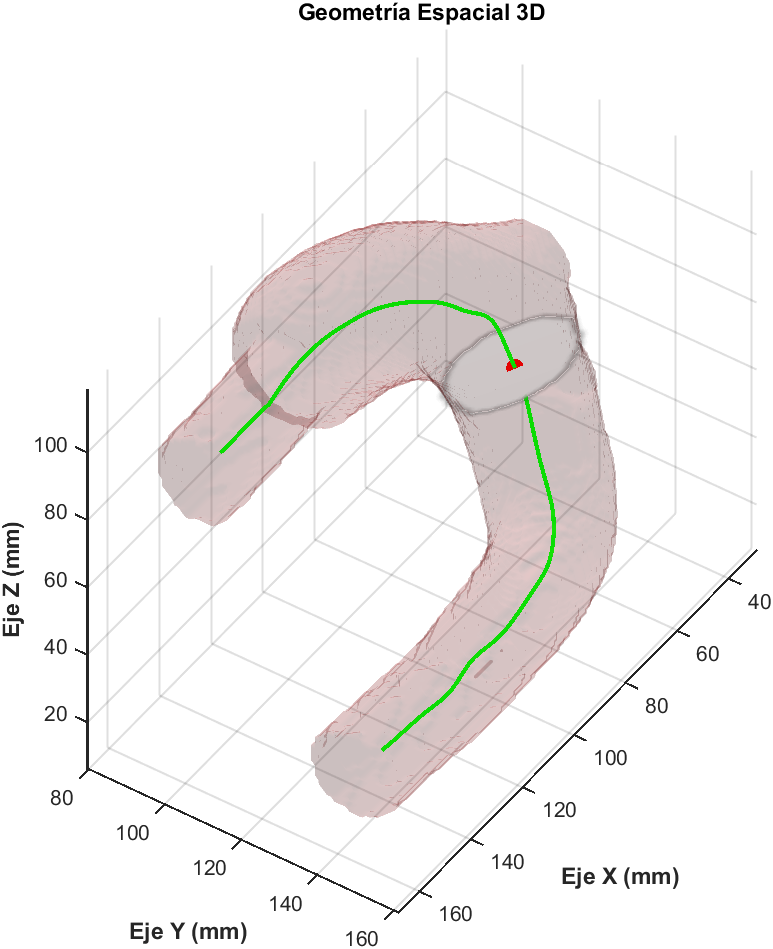
\includegraphics[width=\linewidth]{figures/validacion/fase1/geometria_normal_p45.png}
        \caption{Fantoma normal (Plano 45)}
        \label{fig:geo_normal}
    \end{subfigure}\hfill
    \begin{subfigure}{0.48\textwidth}
        \centering
        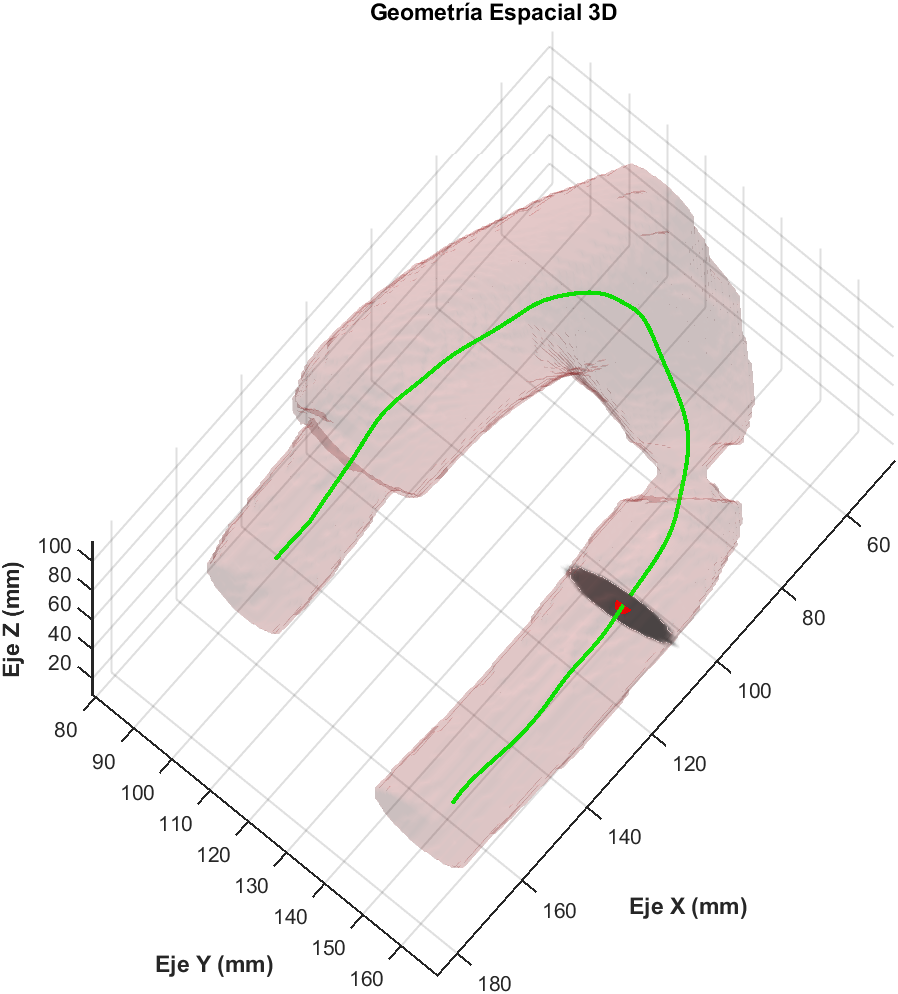
\includegraphics[width=\linewidth]{figures/validacion/fase1/geometria_9mm_p70.png}
        \caption{Fantoma 9 mm (Plano 70)}
        \label{fig:geo_9mm}
    \end{subfigure}
    \caption{Representación espacial tridimensional generada por el sistema. Se evidencia la generación de la isosuperficie, el \textit{centerline} (verde) y el plano transversal de discretización en su respectiva iteración. Destaca la clara captura del estrechamiento en la zona de coartación (b). Fuente: Elaboración propia.}\label{fig:geometrias_fantomas}
\end{figure}

Como se observa en la representación gráfica, el sistema logra integrar la isosuperficie con la discretización del \textit{centerline}, proyectando los planos de corte de manera precisa. La comparación visual confirma la captura de los cambios morfológicos entre fantomas, evidenciando la caída abrupta de diámetro del fantoma con coartación frente a la continuidad del vaso sano.


\subsubsection{Validación de la síntesis acústica y análisis espectral}

Una vez validada la discretización del \textit{centerline}, el flujo de trabajo procede con la proyección de las velocidadades y su transformación en señales sonoras. El objetivo en esta instancia es corroborar que el motor de emulación es capaz de procesar la cinemática aislada y generar exitosamente la síntesis acústica y espectrales.

Para evidenciar la correcta ejecución de esta etapa, la Figura \ref{fig:sintesis_acustica} expone las salidas generadas por el \textit{software} para el fantoma normal (plano 45) y el fantoma con coartación de 9 mm (plano 70).

\begin{figure}[H]
    \centering
    % Fila 1: Espectrogramas
    \begin{subfigure}{0.48\textwidth}
        \centering
        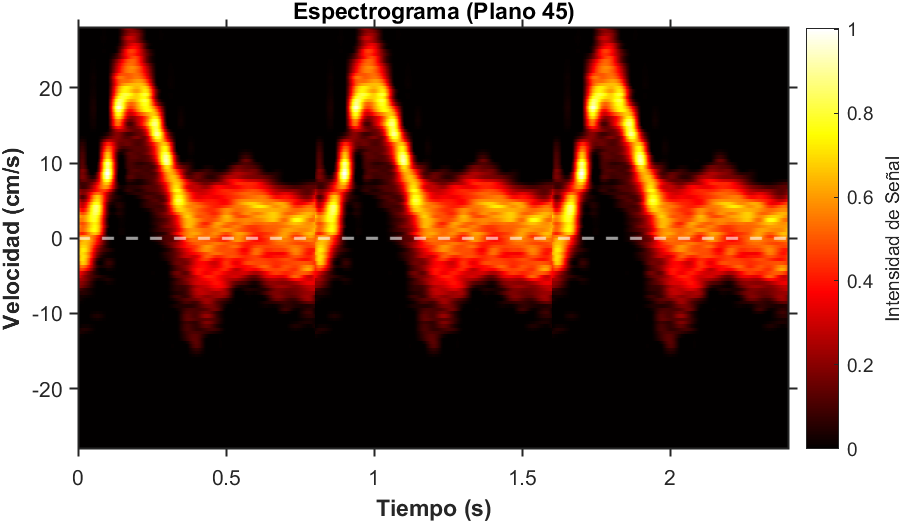
\includegraphics[width=\linewidth]{figures/validacion/fase1/gn_espectro_p45.png}
        \caption{Espectrograma - Fantoma normal}
        \label{fig:spec_normal}
    \end{subfigure}\hfill
    \begin{subfigure}{0.48\textwidth}
        \centering
        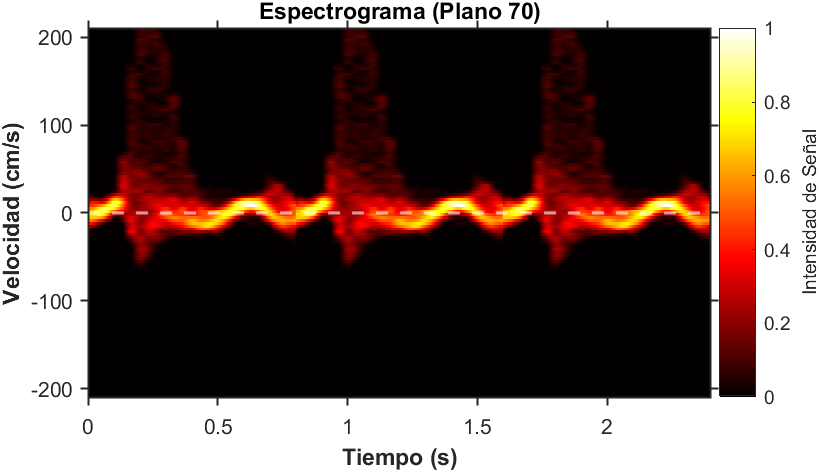
\includegraphics[width=\linewidth]{figures/validacion/fase1/g9_espectro_p70.png}
        \caption{Espectrograma - Fantoma 9 mm}
        \label{fig:spec_9mm}
    \end{subfigure}
    
    \vspace{0.5cm} % Espacio entre filas
    
    % Fila 2: Formas de Onda
    \begin{subfigure}{0.48\textwidth}
        \centering
        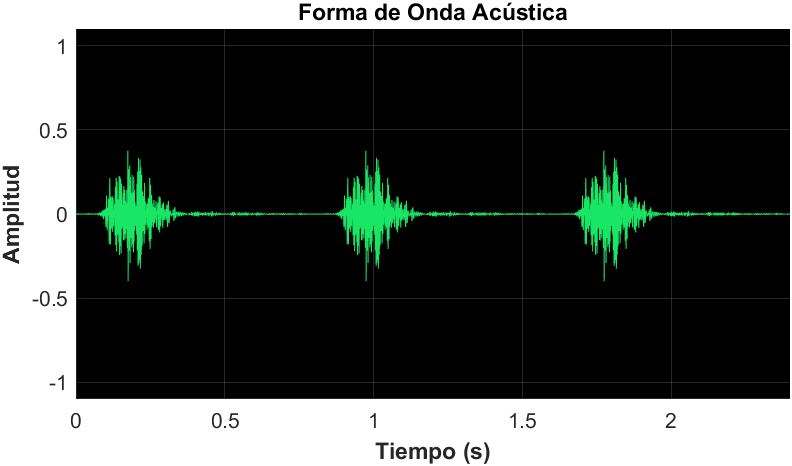
\includegraphics[width=\linewidth]{figures/validacion/fase1/gn_sonido_p45.png}
        \caption{Onda acústica - Fantoma normal (a)}
        \label{fig:onda_normal}
    \end{subfigure}\hfill
    \begin{subfigure}{0.48\textwidth}
        \centering
        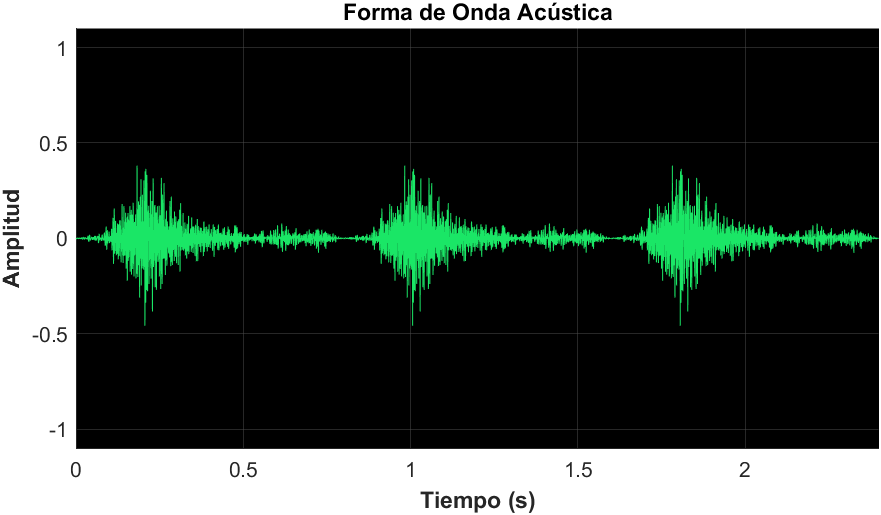
\includegraphics[width=\linewidth]{figures/validacion/fase1/g9_sonido_p70.png}
        \caption{Onda acústica - Fantoma 9 mm (b)}
        \label{fig:onda_9mm}
    \end{subfigure}
    \caption{\label{fig:sintesis_acustica} Espectrograma y onda acústica en condición de reposo (\textit{rest}) para diferentes escenarios morfológicos y topológicos. Fuente: Elaboración propia.}
\end{figure}

Como se observa en los resultados, el sistema logra extraer la información de los planos de corte y traducirla en archivos acústicos y gráficos estructurados. La clara diferencia en las escalas y amplitudes registradas entre ambos modelos confirma que el algoritmo de síntesis responde a los distintos perfiles de velocidad del \textit{4D Flow MRI}, comprobando el correcto desempeño operativo del módulo base. Para complementar esta validación visual, es posible acceder a la reproducción de las señales generadas mediante los siguientes enlaces: \href{https://drive.google.com/file/d/1xQmC3SaCplyq4cFz9ADJMwVXydT0yq6e/view?usp=sharing}{salida acústica del fantoma normal (a)} y \href{https://drive.google.com/file/d/1KgReb6jlhsudJGxGEyWbSvPVMoqxSP4G/view?usp=sharing}{salida acústica del fantoma de 9 mm (b)}.

Complementando la validación espectral y sonora, es necesario comprobar la correcta ejecución del módulo de emulación del \textit{Color Doppler}. Este componente es sirve para corroborar que el algoritmo proyecta adecuadamente los vectores de velocidad de forma dinámica, respondiendo a la evolución fisiológica del ciclo cardíaco sin introducir artefactos topológicos.

A fin de ilustrar esta capacidad, la Figura \ref{fig:validacion_doppler2d_temporal} detalla el mapeo bidimensional de velocidades para el fantoma sin estenosis (Normal) en condición \textit{rest}. La evaluación se focaliza en el plano transversal 45, zona anatómica representativa de la porción central del conducto. Al desplegar esta proyección en cuatro fases discretas del ciclo cardíaco, es posible visualizar la evolución de las proyecciones generadas.

\begin{figure}[H]
    \centering
    % Fila 1
    \begin{subfigure}{0.48\textwidth}
        \centering
        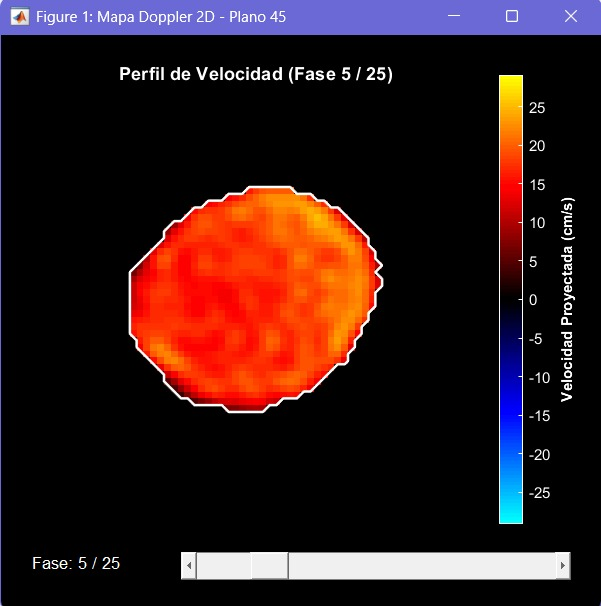
\includegraphics[width=\linewidth]{figures/validacion/fase1/gn_2d_p45_fase5.jpeg} 
        \caption{Fase 5}
        \label{fig:mapa2d_f5}
    \end{subfigure}\hfill
    \begin{subfigure}{0.48\textwidth}
        \centering
        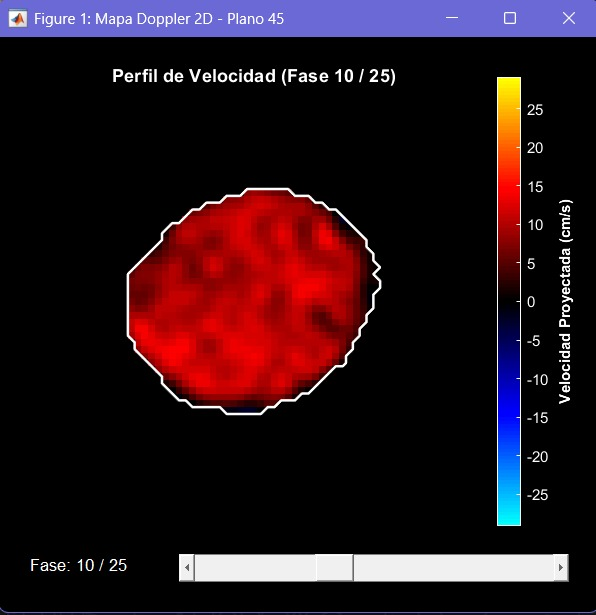
\includegraphics[width=\linewidth]{figures/validacion/fase1/gn_2d_p45_fase10.jpeg} 
        \caption{Fase 10}
        \label{fig:mapa2d_f10}
    \end{subfigure}
    
    \vspace{0.5cm} % Espacio entre filas
    
    % Fila 2
    \begin{subfigure}{0.48\textwidth}
        \centering
        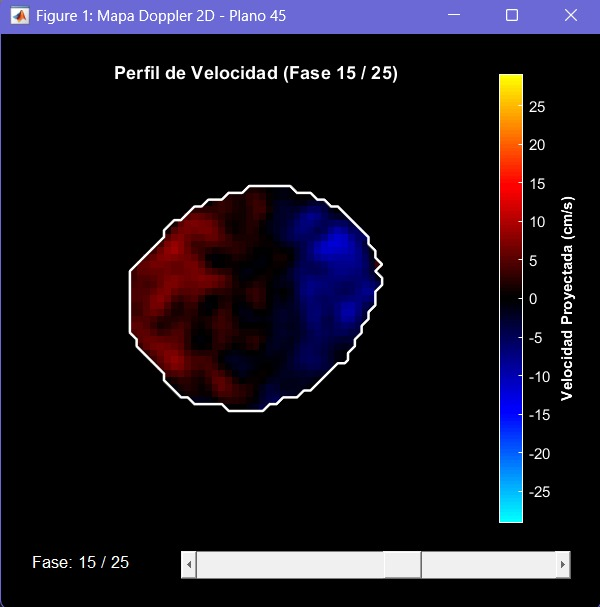
\includegraphics[width=\linewidth]{figures/validacion/fase1/gn_2d_p45_fase15.jpeg} 
        \caption{Fase 15}
        \label{fig:mapa2d_f15}
    \end{subfigure}\hfill
    \begin{subfigure}{0.48\textwidth}
        \centering
        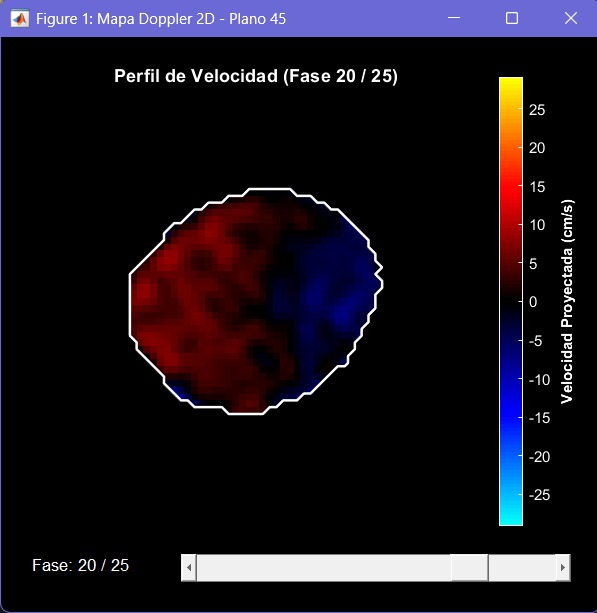
\includegraphics[width=\linewidth]{figures/validacion/fase1/gn_2d_p45_fase20.jpeg} 
        \caption{Fase 20}
        \label{fig:mapa2d_f20}
    \end{subfigure}
    \caption{\label{fig:validacion_doppler2d_temporal} Evolución temporal del \textit{Color Doppler} virtual en el plano 45 del fantoma Normal. Fuente: Elaboración propia.}
\end{figure}

Como se aprecia en la secuencia visual, el sistema aísla exitosamente el plano transversal que atraviesa el vaso, conteniendo exclusivamente los perfiles hemodinámicos de la región de interés. 

En síntesis, el sistema ha demostrado su capacidad para procesar la complejidad de los datos provenientes del \textit{4D Flow MRI}, logrando aislar topológicamente el vaso y traducir su cinemática en representaciones acústicas, espectrales y espaciales consistentes entre sí. No obstante, aunque esta herramienta resulta fundamental para una primera inspección cualitativa, el análisis comparativo entre múltiples morfologías y secciones transversales exige un enfoque paramétrico y escalable. Por consiguiente, la siguiente etapa de validación abordará la segunda fase de la investigación, comprobando cómo este núcleo de procesamiento fue automatizado para extraer, de forma masiva, los descriptores numéricos que caracterizan la hemodinámica de todos los modelos de estudio.


% \subsubsection{Validación de la extracción paramétrica y procesamiento masivo}

% Tras comprobar la fidelidad espacial y acústica del motor base, la validación de la segunda etapa se enfoca estrictamente en verificar el correcto desempeño computacional del algoritmo de procesamiento por lotes (\textit{batch processing}) y la integridad estructural de los datos exportados. El objetivo de esta fase fue procesar de forma ininterrumpida las matrices correspondientes a los diferentes escenarios hemodinámicos para consolidar exitosamente un espacio de características multidimensional, garantizando que el sistema operara de manera autónoma sin pérdida de información.

% El procesamiento continuo de los 8 modelos de estudio (condiciones de reposo y estrés) permitió evaluar un total de 720 secciones transversales anatómicas. Durante la ejecución de esta etapa, la inspección del repositorio intermedio expuso una varianza empírica significativa en la huella de almacenamiento de los archivos. Lejos de representar una anomalía computacional, esta fluctuación constituye una validación geométrica intrínseca: el peso de cada archivo es directamente proporcional al área anatómica de la sección transversal del lumen vascular. Planos amplios contienen un mayor número de vóxeles catalogados como flujo, generando matrices más pesadas, mientras que las zonas estrechas o de coartación producen arreglos sustancialmente más ligeros. Esta correspondencia demuestra que el sistema aísla y se adapta dinámicamente a la morfología real del vaso iteración tras iteración.

% En cuanto a la arquitectura de datos, el diseño computacional priorizó la máxima fidelidad matemática. Durante las etapas preliminares, el sistema operaba los tensores en precisión simple (\textit{single}, 32 bits) para minimizar el impacto en la memoria. No obstante, para evitar errores de truncamiento acumulativos durante la integración de las señales acústicas y el cómputo del espectro de Fourier, se determinó escalar y fijar el procesamiento a precisión doble (\textit{double}, 64 bits). 

% Evidentemente, esta exigencia matemática duplicaba la carga sobre la memoria volátil. Para mitigar este cuello de botella y evitar la saturación de la memoria RAM, se implementó la arquitectura de canalización que exporta de manera fragmentada las matrices de cada plano hacia el almacenamiento local en archivos binarios (\textit{.mat}). Para evidenciar el impacto de esta decisión de ingeniería y la carga que el sistema logró gestionar exitosamente, la Figura \ref{fig:exportacion_batch_precision} contrasta la huella de memoria entre la precisión base y la implementación final de alta resolución.

% \begin{figure}[H]
%     \centering
%     \begin{subfigure}{0.85\textwidth}
%         \centering
%         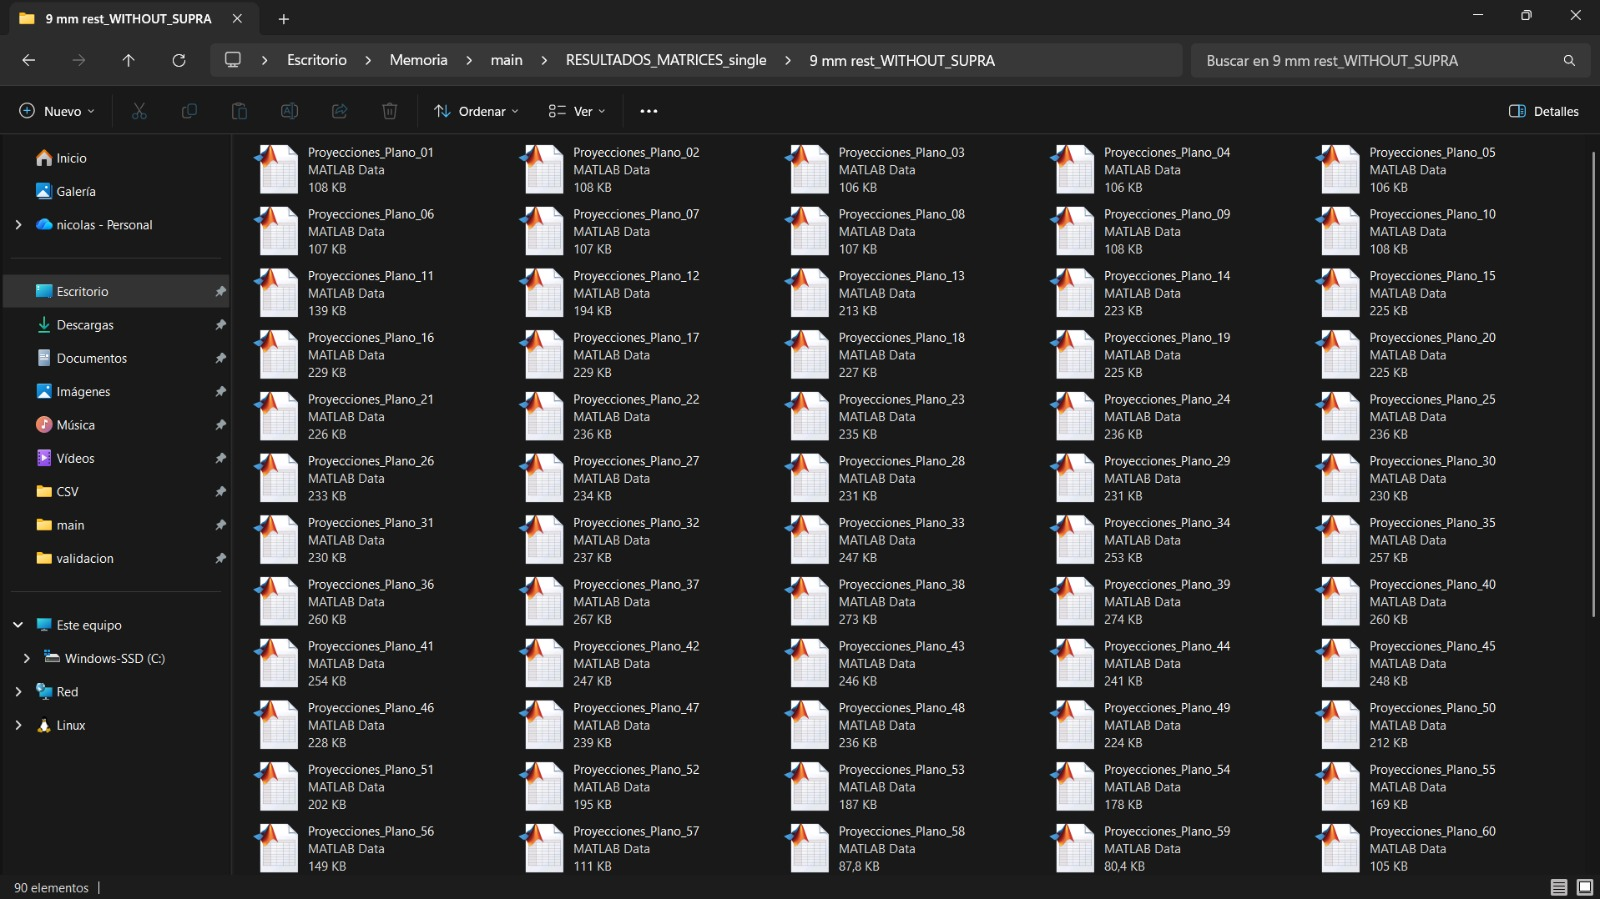
\includegraphics[width=\linewidth]{figures/validacion/fase2/carpetas_single.jpeg} 
%         \caption{Implementación preliminar: Precisión \textit{single} (32 bits)}
%         \label{fig:memoria_single}
%     \end{subfigure}
    
%     \vspace{0.4cm}
    
%     \begin{subfigure}{0.85\textwidth}
%         \centering
%         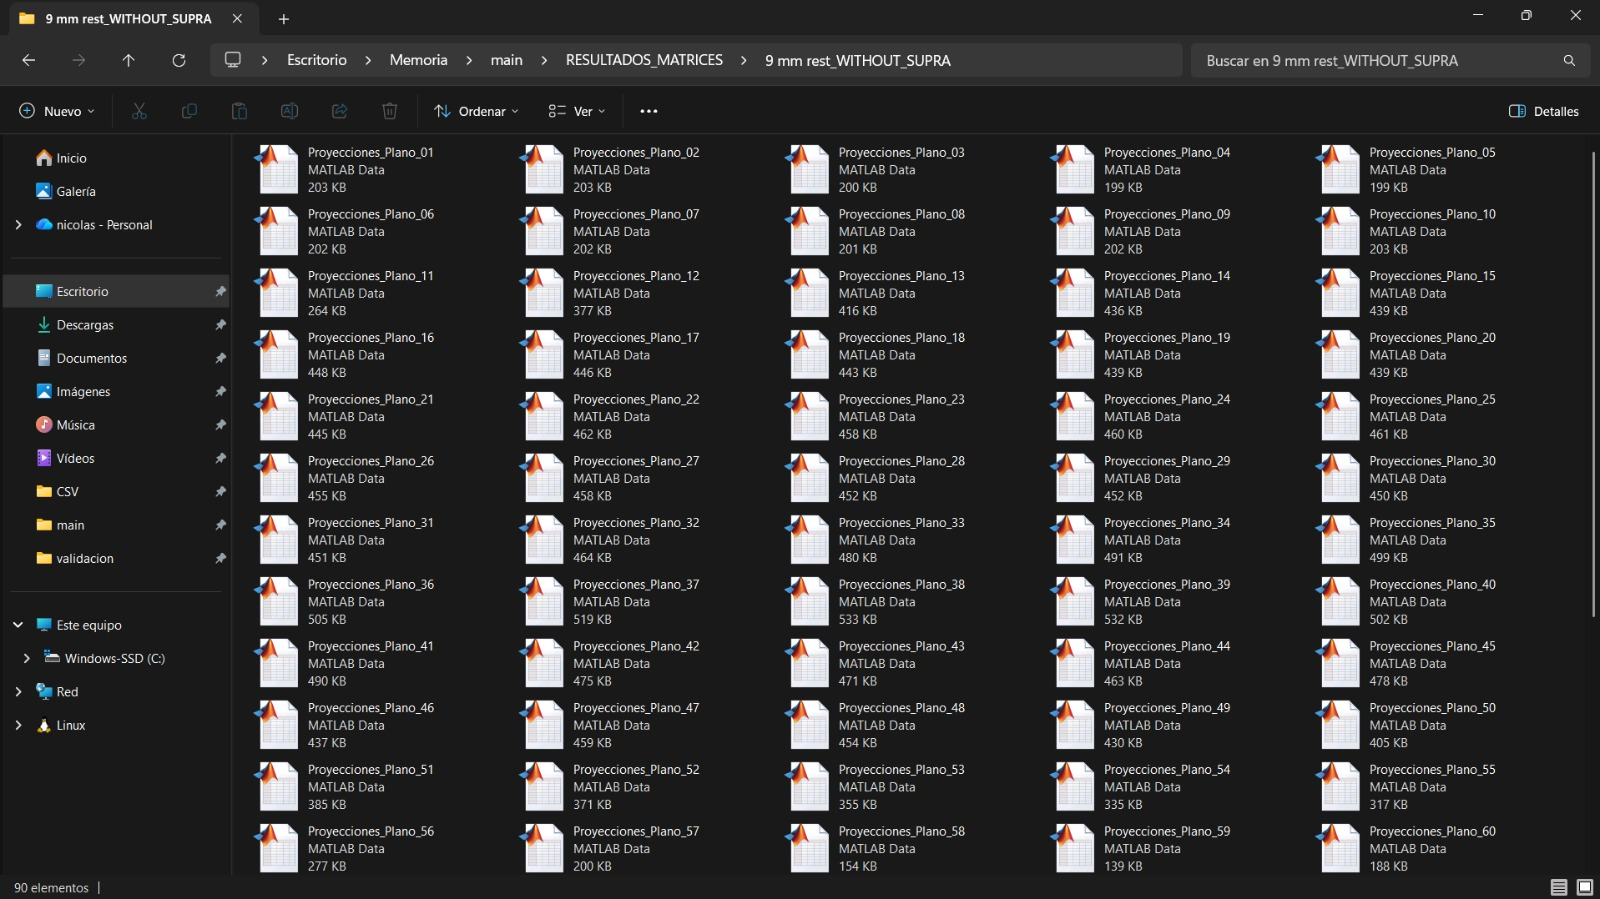
\includegraphics[width=\linewidth]{figures/validacion/fase2/carpetas_double.jpeg} 
%         \caption{Implementación definitiva: Precisión \textit{double} (64 bits)}
%         \label{fig:memoria_double}
%     \end{subfigure}
%     \caption{\label{fig:exportacion_batch_precision} Comparativa del impacto en el almacenamiento local (\textit{Storage Footprint}) generado por el orquestador. El salto hacia la alta precisión (\textit{double}) incrementó el peso por iteración de $\sim$109 KB a $\sim$204 KB; sin embargo, la exportación iterativa evitó la saturación de la RAM, garantizando la máxima integridad para la síntesis acústica. Fuente: Elaboración propia.}
% \end{figure}

% La correcta generación de este repositorio fragmentado y de alta precisión permitió que el módulo de parametrización (\textit{Feature Extraction}) iterara sobre los archivos locales de manera eficiente. El algoritmo extrajo con éxito los descriptores cinemáticos y sonoros para cada plano, culminando en la consolidación de la matriz tabular final (\textit{Dataset}). Esta estructura de datos bidimensional cierra formalmente la etapa de digitalización, sentando las bases numéricas estrictamente necesarias para la validación clínica mediante el descubrimiento de patrones no supervisados.